\documentclass{article}
\usepackage{CJKutf8}
\usepackage{latexsym}
\usepackage{pgfplots}  
\usepackage{pgfplotstable}

\title{Week 1}
\author{软73 沈冠霖 2017013569}
\begin{document}
\begin{CJK}{UTF8}{gkai}
\maketitle

\section{T2} 
证明:$\forall  1 \leq i \leq n,$有B[(i+offset) mod n]=A[i],而offset取1-n之间任意整数的概率都是$\frac{1}{n}$,因此A[i]和B中任意一位相等的概率都是$\frac{1}{n}$。而因此,B只有n种取值可能,不是n!种取值可能,所以无法这样生成全排列。
\section{T3} 
证明:考虑原事件的补集,如果生成的P有重复,则$\exists 1-n$间的整数i,j,使得P[i]=P[j]。给定$i=i_{0},j=j_{0}$,P(P[i]=P[j]) = $\frac{1}{n^{3}}*\frac{1}{n^{3}}*n^{3} = \frac{1}{n^3}$,而根据概率测度的性质,$P(A_{1} \cup A_{2} \cup .....\cup A_{n}) \leq P(A_{1})+P(A_{2})+...+P(A_{n})$,因此原事件补集的概率P(重复)$\leq \frac{1}{2n}-\frac{1}{2n^{2}} \leq \frac{1}{n}$,原事件发生概率P$\geq 1-\frac{1}{n}$

\section{T1} 
\paragraph{测试环境}
CPU:Inter Core i5-6300HQ,2.3GHZ\\
内存:12G\\
环境:VS2017,release模式
\paragraph{第一部分}:比较不同数据规模下暴力算法与分治算法的结果,具体数据见Table 1 与下方折线图。\\
结果分析如下:首先,当数据规模很小(低于1000)的时候,递归算法略快于暴力算法,原因是递归算法在20处停止,相当于只进行了2-4次递归,之后使用暴力算法求解数据规模20的子问题,效率更好。\\
其次,当数据规模中等(1000-30000)的时候,递归算法慢于暴力算法,原因是递归算法有7n的常数,还有递归栈操作等,而在这个时候,递归的次数在5-12次之间,次数已经不小了(递归栈空间成百上千个),因此可能效率降低。\\
最后,数据规模很大(100000+)的时候,递归算法又快了,原因是随着n趋向无穷,f(n) =$\theta$ (nlgn)的递归算法相比f(n) =$\theta (n^{2})$的暴力算法优势又显现出来了。\\
\\
\\
\\

\begin{table}[!htbp] 
	
	\caption{不同数据规模下计算最近两点的时间}
	\begin{flushleft} 
		\begin{tabular}{|l|l|l|l|l|l|l|l|l|l|l|} 
			\hline 测量序号 & 1 & 2 & 3 & 4 & 5 & 6 & 7 & 8\\ 
			\hline 数据范围 &100&300&1000&3000&10000&30000&100000&300000 \\ 
			\hline 第一组(递归到20截止)时间 (ms)
			&2.5&2.8&12.6&35.3&231.5&2559&36847.3&300000  \\
			\hline 第二组(暴力)时间 (ms)
			&4.7&4.7&11.1&27.5&268.7&2379.5&26414.8&458747  \\ 
			\hline 
		\end{tabular} 
		注:每组数据都是运行10次后取的平均值
	\end{flushleft} 
\end{table}


\pgfplotsset{}

	\begin{tikzpicture}

	\begin{axis}[legend pos=outer north east] % 将图例放在图外,位于图的东北角
	\addplot 
	table[]                         
	{           		                
		N T
		100 2.5
		300 2.8
		1000 12.6
		3000 35.3 
	};
	\addplot
	table[] 
	{   				
		N T
		100 4.7
		300 4.7
		1000 11.1
		3000 27.5 
	};
	\addlegendentry{递归算法}         
	\addlegendentry{暴力算法}
	\end{axis}
	\end{tikzpicture}



\pgfplotsset{}

	\begin{tikzpicture}

	\begin{axis}[legend pos=outer north east] % 将图例放在图外,位于图的东北角
	\addplot 
	table[]                         
	{           		                
		N T
		10000 231.5
		30000 2559
		100000 36847.3
		300000 300000
	};
	\addplot
	table[] 
	{   				
		N T
		10000 268.7
		30000 2379.5
		100000 26414.8
		300000 458747
	};
	\addlegendentry{递归算法}         
	\addlegendentry{暴力算法}
	\end{axis}
	\end{tikzpicture}


\paragraph{第二部分}:对于n=10000的情形,比较在不同取值m时,停止递归进行暴力求解的程序运行时间,具体数据见Table 2 与下方折线图。\\
分析:首先,当m很小(m$\leq$ 20)的时候,因为此时递归层数已经有 10-15层,递归栈的大小,栈操作的时间等随递归层数指数增长,因此递归还不如暴力快。\\
其次,当m中等($50\leq m\leq 1000$),当递归层数<8层的时候,递归的效率已经高于暴力了。当m在500-1000间,也就是递归3-4层的时候,递归效率大致达到最高。此时,递归降低时间复杂度的优点和常数大,栈内存操作多的劣势达到了平衡\\
最终,当m较大(m $\geq$ 2000)的时候,虽然递归还是能明显提高速度,但是因为层数太小,没有把子问题分解的足够小,因此效率还是不高。\\
综上,可以看出,在实际情况下,如果要用递归的方法优化一个程序,我们需要平衡好递归的优点(降低时间复杂度)和缺点(栈内存各种操作太慢)等,对于10000这个数据规模而言,3-4次递归是最好的。



\begin{table}[!htbp] 
	
	\caption{n=10000时,不同递归终止条件消耗的时间}
	\begin{flushleft} 
		\begin{tabular}{|l|l|l|l|l|l|l|l|l|l|l|} 
			\hline 测量序号 & 1 & 2 & 3 & 4 & 5 & 6 & 7 & 8& 9&10\\ 
			\hline 递归截止的数据大小m &1&5&10&20&50&100&500&1000&2000&10000(不递归) \\ 
			\hline 时间 (ms)
			&3842.5&814.1&410.4&219.8&115.8&64&29.1&29.8&41.1&268.7  \\ 
			\hline 
		\end{tabular} 
		注:每组数据都是运行10次后取的平均值
	\end{flushleft} 
\end{table}


\pgfplotsset{}

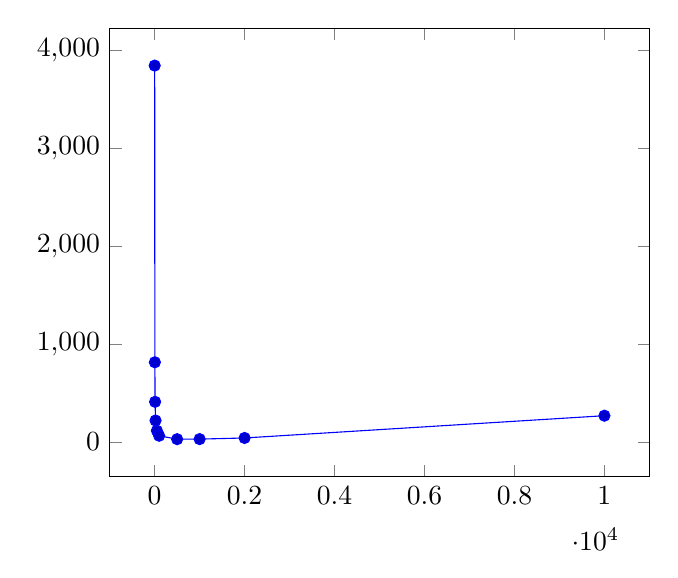
\begin{tikzpicture}

\begin{axis}[legend pos=outer north east] % 将图例放在图外,位于图的东北角
\addplot 
table[]                         
{           		                
	N T
	1 3842.5
	5 814.1
	10 410.4
	20 219.8
	50 115.8
	100 64
	500 29.1
	1000 29.8
	2000 41.4
	10000 268.7

};


\end{axis}
\end{tikzpicture}


\end{CJK}
\end{document}
